\documentclass[]{article}
\usepackage[utf8]{inputenc}
\usepackage{pdfpages}
\usepackage{amsmath}
\usepackage{amssymb}
\usepackage{graphicx}
\usepackage{geometry}
\usepackage{enumitem}
\usepackage{amsthm}

\usepackage{graphicx}
\usepackage{geometry}

\geometry{hmargin=2cm}

\title{Analyse}

\author{Isabelle Galagher et Pierre Gervais}

% Environnement type théorème
\newtheorem{mythm}{Théorème}
\newtheorem{myproposition}{Proposition}
\newtheorem{myproperty}{Propriété}
\newtheorem{mylemma}{Lemme}
\newtheorem{mycor}{Corollaire}

% Environnement type texte
\theoremstyle{remark}
\newtheorem{mynot}{Notation}
\newtheorem{myrem}{Remarque}
\newtheorem{myexer}{Exercice}
\newtheorem{myproof}{Preuve}
\newtheorem{myexmpl}{Exemple}

% Environnement de définition
\theoremstyle{definition}
\newtheorem{mydef}{Définition}

\setlist[itemize]{label=-}

% Carré de fin de preuve
\newcommand{\cqfd}{
	\hfill$\square$
}

% "Checkmark" de fin d'étape de preuve
\newcommand{\checked}{
	\hfill$\checkmark$
}

% Définition de fonction
\newcommand{\func}[5]{
#1 ~ : ~ \left\{ \begin{array}{lcl}
	#2 & \longrightarrow & #3 \\
	#4 & \longmapsto & #5
\end{array}
\right.
}

\newcommand{\funcinline}[5]{
#1 ~ : ~ #2 \longrightarrow #3, ~ #4 \longmapsto #5
}

\newcommand{\funcshort}[3]{
#1 ~ : ~ #2 \longrightarrow #3
}

\newenvironment{proofpart}[1]{
	\leavevmode
	
	\noindent
	{\textit{\textbf{\boldmath #1}}}
	
}{
	\checkmark
}

\begin{document}

\maketitle

\tableofcontents

\part{Topologie des espaces vectoriels normés}

\section{Espaces vectoriels normés : premières définitions}

\subsection{Distances et normes}

\begin{mydef}
	Étant donné un ensemble $E$, une \textit{distance sur $E$} est une application $d~: ~ E \times E \longrightarrow \mathbb{R}$ vérifiant les propriétés suivantes :
	\begin{enumerate}
		\item $d$ est \textit{définie positive} : $d(x,y) \geqslant 0$ et $d(x,y) = 0 \Leftrightarrow x=y$
		\item $d$ est symétrique : $d(x,y)=d(y,x)$
		\item $d$ vérifie l'\textit{inégalité triangulaire} : $\forall z \in E, ~ d(x,y) \leqslant d(x,z) + d(z, y)$
	\end{enumerate}
\end{mydef}

\begin{myexmpl}
	\leavevmode
	\begin{itemize}
		\item $E=\mathbb{R}$ et $d(x, y) = |x-y|$
		\item $E=\mathbb{R}^2$ et $d\left(\binom{a}{b},\binom{c}{d}\right)=\sqrt{(a-c)^2+(b-d)^2}$
	\end{itemize}
\end{myexmpl}

\begin{myrem}
	Par l'inégalité triangulaire, on déduit
	\begin{itemize}
		\item $d(x,z) \geqslant d(x, y) - d(y, z)$
		\item $d(x, z) \geqslant d(z, y) - d(x, y)$
	\end{itemize}
	d'où $|d(x, y) - d(z, y)| \leqslant d(x, z)$
\end{myrem}

\begin{mydef}
	Soit $E$ un $\mathbb{K}$-espace vectoriel, une \textit{norme} sur $E$ est une application notée $N$ ou $\|\cdot\|$ telle que
	\begin{enumerate}
		\item $(x, y) \longmapsto \|x - y\|$ est une distance
		\item $\forall \lambda \in \mathbb{R}, ~ \forall u \in E, ~ \|\lambda u\| = |\lambda|\|u\|$ (\textit{homogénéité})
	\end{enumerate}
\end{mydef}

\begin{myproposition}
	Une fonction $\|\cdot\| ~ : ~ E \longrightarrow \mathbb{R}$ est une norme si et seulement si :
	\begin{enumerate}
		\item elle est homogène
		\item elle est définie
		\item elle vérifie l'inégalité triangulaire
	\end{enumerate}
\end{myproposition}

\begin{myproof}
	\leavevmode
	
	{\boldmath $\Longrightarrow$}
	
	Soit $\|\cdot\|$ une norme.
	\begin{enumerate}
		\item \checkmark
		\item $\|x\|=d(x, 0)$ où $d(x,y)=\|x-y\|$, donc $\|x\| \geqslant 0$ et $\|x\|=0 \Longleftrightarrow d(x, 0)=0 \Longleftrightarrow x=0$
		\item $\|x+y\| = d(x+y, 0) = d(x, -y)$, or $\forall x, y, z \in E, ~ d(x, z) \leqslant d(x, y) + d(y, z)$ donc $d(x, -y) \leqslant d(x, 0) + d(0, -y)$
		D'où $\|x+y\| \leqslant d(x, 0) + d(0, -y) \leqslant \|x\| + \|-y\| \leqslant \|x\| + \|y\|$
	\end{enumerate}
	
	{\boldmath $\Longleftarrow$}
	
	Soit $\| \cdot \|$ vérifiant les trois propriétés, alors soit $d(x, y)=\|x-y\|$ et montrons que d est une distance.
	
	\begin{enumerate}
		\item $d(x, y) \geqslant 0$ car $\|x-y\| \geqslant 0$ par (2).
		$d(x, y) = 0 \Longleftrightarrow \|x-y\| = 0 \Longleftrightarrow x = y$
		
		\item $d(x, y) = \|x-y\|=\|-(x-y)\| = \|y-x\|=d(y, x)$
		
		\item $d(x, y) = \|x-y\| = \|x-z + z - y\| \leqslant \|x-z\| +\|z-x\| \leqslant d(x, y) + d(z, y)$
 	\end{enumerate}
 	\cqfd
\end{myproof}

\begin{myexmpl}
	\leavevmode
	\begin{enumerate}
		\item Dans $\mathbb{R}^n$, on définit les normes $\displaystyle \|x\|_1= \sum_{k=1}^n |x_k|$, $\displaystyle \|x\|_2 =  \sqrt{\sum_{k=1}^n |x_k|^2}$, $\displaystyle \|x\|_p = \sqrt[p]{\sum_{k=1}^n |x_k|^p}$ et $\displaystyle \|x\|_\infty = \max_{k} \|x_k\|$
		\item Dans $\mathbb{R}^n$ muni d'un produit scalaire, $\|x\| = \sqrt{\langle x, x\rangle}$
		\item Soit $A$ un ensemble et $F$ une espace vectoriel normé, et $\mathcal{B}(A, F)$ les fonctions bornées de $A$ dans $F$, alors $\displaystyle \|f\|_\infty = \sup_{x \in A} \|f(x)\|$ est une norme.
		\item Sur $\mathcal{C}([0, 1], \mathbb{R})$, $\displaystyle \|f\|_1 = \int_{0}^{1}\left|f(x)\right|$, $\displaystyle \|f\|_2 = \sqrt{\int_{0}^{1}\left|f(x)\right|^2}$ et$\displaystyle \|f\|_\infty = \sup_{0 \leqslant x \leqslant 1}\left|f(x)\right|$
	\end{enumerate}
\end{myexmpl}

\begin{mydef}
	Deux normes $N_1$ et $N_2$ sont dites \textit{équivalentes} s'il existe des constantes strictement positives $C_1$ et $C_2$ telles que $\forall x \in E, ~ C_1 N_2(x) \leqslant N_1(x) \leqslant C_2 N_2(x)$
\end{mydef}

\begin{myexmpl}
	Par exemple dans $\mathbb{R}^n$, les normes $\|\cdot\|_1$, $\|\cdot\|_2$ et $\|\cdot\|_\infty$ sont équivalentes. En effet $$\|x\|_1=|x_1|+|x_2| \leqslant 2 \|x\|_\infty$$ et $\|x_i| \geqslant \|x\|_\infty, ~ i=1, 2$
\end{myexmpl}

En dimension finie, toutes les normes sont équivalentes ! Cela n'est en revanche pas vraie en dimension infinie.

\begin{figure}[h!]
	\centering
	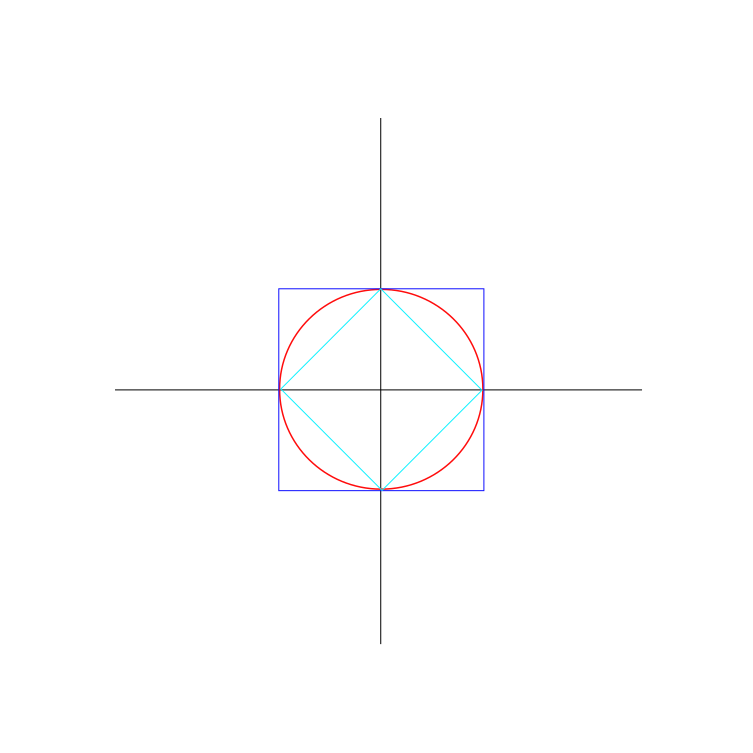
\includegraphics[width=350pt]{Schema1}
	\caption{Différentes boules unités}
	En bleu : $\mathcal{B}_\infty(0, 1)$
	
	En rouge : $\mathcal{B}_2(0, 1)$
	
	En turquoise : $\mathcal{B}_1(0, 1)$
\end{figure}

\subsection{Ouverts et fermés}

\begin{mydef}
	Soit $E$ un espace vectoriel normé, on appelle \textit{boule fermée} de centre $x$ et de rayon $r > 0$ l'ensemble $\overline{\mathcal{B}}(x, r) = \{u \in E ~|~ \|x-u\| \leqslant r\}$, et la \textit{boule ouverte} de centre $x$ et de rayon $r > 0$ l'ensemble $\mathcal{B}(x, r) = \{u \in E ~|~ \|x-u\| < r\}$.
\end{mydef}

\begin{mydef}
	Soit $X \subseteq E$
	\begin{enumerate}
		\item On dit que $U \subseteq X$ est un \textit{ouvert} de $X$ si $\forall x \in U, ~ \exists r > 0 ~ : ~ \mathcal{B}(x, r) \cap X \subseteq U$
		\item On dit que $F \subseteq X$ est un \textit{fermé} de $X$ si son complémentaire dans $X$ est un ouvert de $X$.
	\end{enumerate}
\end{mydef}

\begin{figure}[h!]
	\centering
	\includegraphics[width=200pt]{Ouverts_fermes}	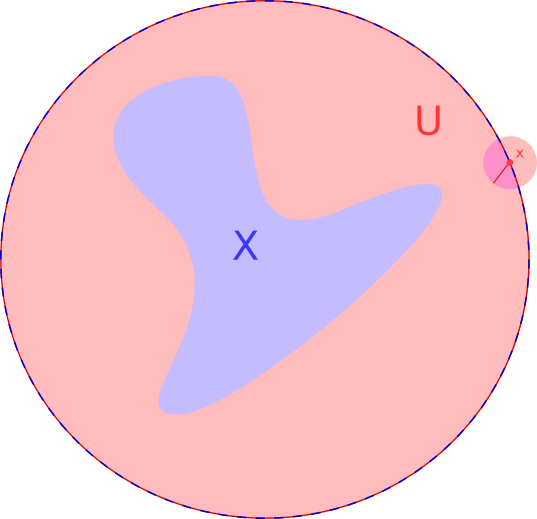
\includegraphics[width=200pt]{Ouverts_fermes2}
	\caption{Deux exemples d'ouverts}
\end{figure}

\begin{myrem}
	\leavevmode
	\begin{enumerate}
		\item Un ouvert dans $X$ n'est pas nécessairement ouvert dans $E$, comme montré dans le deuxième exemple de la figure ci-dessus.
		\item Un ouvert de $E$ sera appelé un \textbf{ouvert}, de même pour les fermés.
		
		\item Toute boule ouverte est un ouvert.
		
		\item Toute boule fermée est un fermé.
	\end{enumerate}
\end{myrem}

\newpage

\begin{myproof}
	On considère une boule ouverte $\mathcal{B}(x_0, r)$, montrons que c'est un ouvert.
	
	Soit $x \in \mathcal{B}(x_0, r)$, alors $\|x-x_0\| < r$. On cherche $r'$ tel que $\mathcal{B}(x, r') \subseteq \mathcal{B}(x_0, r)$ donc $r'$ doit vérifier $$\|x-y\| < r' \Longrightarrow \|x_0-y\| < r$$.
	
	Mais $\|x_0-y\| \leqslant \|x-y\| + \|x-x_0\| < \|x-y\| + r$.
	
	Soit $\delta = r - \|x-x_0\| > 0$, on pose alors $r'=\frac{\delta}{2} > 0$, alors $\|x_0-y\| \leqslant r' + \|x-x_0\| \leqslant r' + r - \delta < r$

	\cqfd
\end{myproof}

\begin{figure}[h!]
	\centering
	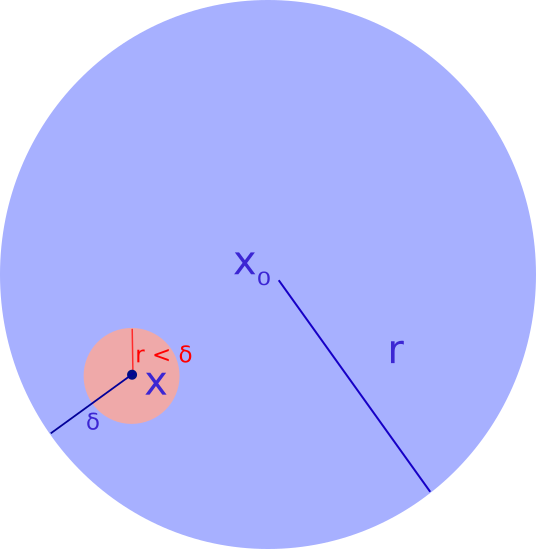
\includegraphics[width=350pt]{Schema2}
	\caption{Construction de la boule ouverte}
\end{figure}

\begin{myproposition}
	L'intersection de deux ouverts est un ouvert et toute réunion d'ouverts est un ouvert.
\end{myproposition}

\begin{myproof}
	Soient $U$ et $U'$ deux ouverts, montrons que $U \cap U'$ est un ouvert.
	
	Soit $x \in U \cap U'$, il existe $r>0$ et $r'>0$ tels que $\mathcal(B)(x, r) \subseteq U$ et $\mathcal{B}(x, r') \subseteq U'$.

	On pose $\widetilde{r}=\min(r, r')$ et on a $\mathcal{B}(x, \widetilde{r}) \subseteq U \cap U'$
	
	\cqfd
\end{myproof}

\begin{myproof}
	Soit $(U_i)_{i \in I}$ une famille d'ouverts, montrons que $U = \displaystyle \bigcup_{i \in I} U_i$ est un ouvert.
	
	Soit $x \in U$, alors il existe $i_0 \in I$ tel que $x \in U_{i_0}$, il existe donc $r$ tel que $\mathcal{B}(x, r) \subseteq U_{i_0}$ car $U_{i_0}$ est ouvert, d'où $\mathcal{B}(x, r) \subseteq U$.
	
	\cqfd
\end{myproof}

\begin{myproposition}
	Soit $X \subseteq E$, tout ouvert $U$ de $X$ s'écrit sous la forme $U=X \cap \widetilde{U}$, où $\widetilde{U}$ est un ouvert.
	
	De même pour tout fermé $F$ de $X$ s'écrit $F=X \cap \widetilde{F}$ où $\widetilde{F}$ est un fermé.
\end{myproposition}

\begin{myproof}
	Soit $\widetilde{U}$ un ouvert de $E$, alors $\widetilde{U} \cap X$ est un ouvert de $X$ par construction.
	
	Inversement soit $U$ ouvert de $X$, alors $\forall x \in U, ~ \exists r(x) > 0$ tel que $\mathcal{B}(x, r(x)) \cap X \subseteq U$
	
	Soit alors $\displaystyle \widetilde{U} = \bigcup_{x \in U} \mathcal{B}(x, r(x))$, alors $\widetilde{U}$ est un ouvert et $U = X \cap U$
	\cqfd
\end{myproof}

\begin{mydef}
	Une suite à valeurs dans $E$ est dite \textit{convergente vers $x \in E$} si pour tout $\epsilon > 0$ il existe un rang $N$ tel que pour tout $n \geqslant N$ on ait $\|x_n-x\| < \epsilon$.
	
	Celle-ci est unique et on la note $\lim\limits_{n} x_n = x$.
\end{mydef}

On remarquera qu'une suite convergente est bornée.

\begin{myproof}
	Soient $x$ et $y$ deux limites de la suite convergente $(x_n)_n$.
	
	Pour tout $\epsilon > 0$ on peut trouver un rang $N$ à partir duquel $\|x_n-x\|<\epsilon$ et $\|y_n-x\|<\epsilon$, d'où
	
	$$\|x-y\| \leqslant \|x-x_n\| + \|x_n-y\| < 2\epsilon$$
	
	Cette inégalité est vraie pour tout $\epsilon>0$ donc $x=y$.
	
	\cqfd
\end{myproof}

\begin{myrem}
	On rappelle que dans $\mathbb{R}$, toute suite majorée croissante est convergente.
	
	Soit $A=\{x_n ~ | ~ n \geqslant 0\}$, et on note $l = \sup A$.
	
	Soit $\epsilon > 0$, $l - \epsilon$ ne majore pas $A$ donc il existe un rang $N$ à partir duquel $x_n \geqslant l-\epsilon$, mais on a aussi $x_n \leqslant l$ pour tout $n$, on a ainsi à partir de $N$ l'encadrement $l - \epsilon \leqslant x_n \leqslant l + \epsilon$.
	
	On a de plus que $\lim\limits_{n} x_n = \sup \{x_n | n \geqslant 0\}$
\end{myrem}

\begin{myrem}
	Si une suite est convergente pour une norme, alors elle l'est pour toute norme équivalente à celle-ci.
	
	Cela n'est pas vrai en général si les normes ne sont pas équivalentes.
	
	Sur l'ensemble des fonctions continue sur $[0, 1]$ on définit les normes
	
	$$\|f\|_{\infty} = \sup_{[0,1]} |f(x)| \text{ et } \|f\| = \int_{0}^{1} |f|$$
	
	On considère la suite de fonction $f_n ~ : ~ x \longmapsto x^n$, on a $$\displaystyle \|f_n\|_{\infty} = \sup_{[0, 1]} |f_n(x)| = 1$$ mais $\|f_n\|=\int_{0}^{1}x^ndx=\frac{1}{n+1} \longrightarrow 0$, les normes ne sont pas équivalentes.
\end{myrem}

\begin{mydef}
	On appelle \textit{valeur d'adhérence} de $x_n$ toute limite d'une sous-suite (suite extraite) de $(x_n)$.
	
	Et on appelle \textit{point d'accumulation} d'une suite $(x_n)$ un point $x$ tel que $\forall \epsilon > 0, ~ \forall N, ~ \exists n > N ~ : ~ \|x_n-x\| < \epsilon$.
\end{mydef}

\begin{myproposition}
	Tout point d'accumulation d'une suite convergente $(x_n)$ est une valeur d'adhérence, et réciproquement.
\end{myproposition}

\begin{myproof}
	\begin{proofpart}{Valeur d'adhérence $\Longrightarrow$ point d'accumulation :}
	
		Soit $x$ une valeur d'adhérence de $(x_n)$, il existe une fonction entière strictement croissante $\phi$ telle que $$\forall \epsilon > 0, ~ \exists N ~ : ~ \forall n > N, ~ \|x_{\phi(n)}-x\| < \epsilon$$
		donc $x$ est un point d'accumulation.
	\end{proofpart}
	
	\begin{proofpart}{Point d'accumulation $\Longrightarrow$ valeur d'adhérence :}
		Réciproquement, soit $x$ un point d'accumulation d'une suite $(x_n)$, on construit par récurrence $\phi$ telle que $x$ soit la limite de $(x_{\phi(n)})_n$ par 
		
		$$
		\phi(n) = \left\{
			\begin{array}{ll}
				0, ~ n = 0 \\
				\min\{k > \phi(n-1) ~ | ~ \|x_k-x\| < 2^{-n}\}, ~ n > 0
			\end{array}
		\right.
		$$
		
		L'application est bien strictement croissante.
		
		Montrons à présent que $y_n=x_{\phi(n)}$ converge vers $x$ : 
		
		soit $\epsilon \in ]0, 1[$, on cherche $N$ tel que pour tout $n > N, ~ \|x_n-x\| < \epsilon$.
		
		Pour $N > \frac{\ln \epsilon}{\ln 2}$ on a $$\forall n > N, ~ \|y_n-x\| < 2^{-n} < \epsilon$$
		
		$(y_n)_n$ est bien une suite convergeant vers $x$.
	\end{proofpart}
	
\end{myproof}

\begin{myproposition}
	Soit $E$ un espace vectoriel normé et $F \subseteq E$.
	
	F est fermé \textit{si et seulement si} $F$ contient la limite de toutes ses suites convergentes.
\end{myproposition}

\begin{myproof}
	\begin{proofpart}{$F$ fermé $\Longrightarrow$ $F$ contient les limites de ses suites}

		Soit $(x_n)$ une suite convergente de $F$ de limite $x$. Montrons que $x \in F$.
		
		Supposons par l'absurde $x \not \in F$, alors $x \in (E \verb|\| F)$ qui est ouvert. Il existe donc $r > 0$ tel que $\mathcal{B}(x, r) \subseteq (E \verb|\|F)$, mais il existe un rang à partir duquel $\|x_n-x\| < \frac{r}{2}$, c'est à dire $x_n \in \mathcal{B}(x, r)$, ce qui contredit $\mathcal{B}(x, r) \subseteq (E \verb|\| F)$.
	\end{proofpart}
	
	
	\begin{proofpart}{$F$ contient les limites de ses suites $\Longrightarrow$ $F$ est fermé}
	
		On suppose à présent que $F$ contient la limite de toute ses suites convergentes, montrons que $F$ est fermée, donc que $E \verb|\|F$ est ouvert.
		
		Soit $x \in (E \verb|\|F)$, montrons qu'il existe $r > 0$ tel que $\mathcal{B}(x, r) \subseteq (E \verb|\|F)$.
		
		Supposons que pour tout $n$, $\mathcal{B}\left(x, \frac{1}{n}\right) \not \subseteq (E \verb|\| F)$, c'est à dire quil existe $x_n \in F$ tel que $x_n \in \mathcal{B}\left(x, \frac{1}{n}\right)$
		
		On a ainsi construit une suite de $F$ convergente vers $x \in F$, donc par hypothèse $x \in F$, ce qui contredit le fait que $x$ appartienne au complémentaire de $F$.
	\end{proofpart}
	
	\cqfd
\end{myproof}

\begin{mydef}
	Soit $X$ une partie d'un espace vectoriel normé $E$.
	
	\begin{itemize}
	\item \textit{L'intérieur de $X$} est le plus grand ouvert inclus dans $X$ noté $\mathring{A}$.
	
	\item \textit{L'adhérence de $X$} est le plus petit fermé contenant $X$ noté $\overline{X}$.
	
	\item \textit{La frontière de $X$} est l'ensemble $\partial X=Fr(X)=\overline{X} \verb|\| \mathring{X}$
	\end{itemize}
\end{mydef}

\begin{myexmpl}
	Si $X = ]0, 1]$ sur $\mathbb{R}$ alors $\mathring{X} = ]0, 1[$, $\overline{X}=[0, 1]$ et $Fr(X)=\{0, 1\}$.
\end{myexmpl}

\begin{myrem}
	X est ouvert si est seulement si $\mathring{X} = X$ et $X$ est fermé si et seulement si $\overline{X}=X$.
\end{myrem}

\begin{myexer}
	Le montrer.
\end{myexer}

\begin{myproof}Intérieur
	
	Soit $\mathring{X}$ l'ensemble des $x \in X$ tels qu'il existe $r > 0$ tel que $\mathcal{B}(x, r) \subseteq X$, alors $\mathring{X}$ est la réunion de tous les ouverts contenus dans $X$.
	
	En effet, $\mathring{X}$ est ouvert dans $X$ par définiton, donc $\mathring{X} \subseteq \text{"réunion des ouverts de X"}$.
	
	Soit $U$ un ouvert de $X$, montrer que $U \subseteq X$.
	
	Soit $x \in U$, il existe $r>0$ tel que $\mathcal{B}(x, r) \subseteq U$ ar $U$ est ouvert. Donc $x \in \mathring{X}$.
	
	$\mathring{X}$ est donc ouvert, contenu dans $X$. Il contient tous les ouverts de $X$, donc c'est le plus grand de $X$, d'où le résultat.
	\cqfd
\end{myproof}

\begin{myproposition}
	On caractérise l'adhérence d'une partie $X$ comme étant l'ensemble des limites de sous-suites de $X$.
\end{myproposition}

\begin{myproof}
	Soit $A$ l'ensemble des limites de suites convergentes à valeurs dans $X$.
	
	
	\begin{proofpart}{$A$ est un fermé contenant $X$}
		Pour tout $x \in X$, $x$ peut être la limite d'une suite à valeur dans $X$, c'est à dire $x \in A$ et donc $X \subseteq A$.
		
		Cela signifie en particulier que $A$ contient les limites de ses suites : c'est un fermé.
	\end{proofpart}
	
	\begin{proofpart}{$A$ est le plus petit fermé contenant X}
		Supposons que $A$ ne soit pas minimal, soit $B$ un fermé vérifiant
		$$
			\left\{
			\begin{array}{l}
				X \subseteq B\\
				B \subsetneq A
			\end{array}\right.$$
		
		Il existe donc $a \in A$ tel que $a \not\in B$, c'est à dire la limite d'une suite $(a_n)_n$ à valeurs dans $X$.
		
		Or $B$ est un fermé, donc il contient la limite de ses suites, dont $(a_n)$, donc $a \in B$ : \textbf{contradiction}.
		
		$A$ est donc minimal.
	\end{proofpart}
	
	$A$ est donc le plus petit fermé contenant $X$, c'est à dire $A = \overline{X}$	
\end{myproof}

\section{Applications continues}

\begin{mydef}
	Soient $E$ et $F$ deux espaces vectoriels normés, soient $X \subseteq E$, $Y \subseteq F$ et $f$ une application de $X$ dans $Y$.
	
	On dit que $f$ est continue en un point $x \in X$ si $$\forall \epsilon > 0, \exists \delta > 0 ~ : ~ (\forall u, ~ \|x-u\| < \delta \Longrightarrow \|f(x)-f(u)\| < \epsilon)$$
\end{mydef}

\begin{mythm}
	Une application $f~:~X \longrightarrow Y$ est continue en $x_0 \in X$ si et seulement si pour toute suite $(y_n)$ convergeant vers $x_0$, la suite $\left(f(y_n)\right)_n$ converge vers $f(x_0)$.
\end{mythm}

\begin{myexer}
	Le démontrer
\end{myexer}

\begin{mythm}
	Soit une application $f~:~X \longrightarrow Y$, les assertions suivantes sont équivalentes :
	\begin{enumerate}
	 \item $f$ est continue sur $X$
	 \item l'image réciproque de tout ouvert de $Y$ est un ouvert de $X$
	 \item l'image réciproque de tout fermé de $X$ est une fermé de $X$.
 	\end{enumerate}
\end{mythm}

\begin{myproof}
	\begin{proofpart}{1. $\Longrightarrow$ 2.}
		Soit $f$ continue sur $X$ et $U$ un ouvert de $Y$. Montrer que $f^{-1}(U)=V$ est un ouvert de $X$.
		
		Soit $x \in f^{-1}(U)$, alors $f(x) \in U$, il existe donc $r>0$ tel que $\mathcal{B}(f(x), r) \subseteq U$.
		
		Or il existe $\delta > 0$ tel que pour $\|x-u\| < \delta$, on a $\|f(x)-f(y)\| < \frac{r}{2}$.
		
		Ainsi si $y \in \mathcal{B}\left(x, \frac{\delta}{2}\right)$ alors $f(y) \in \mathcal{B}(f(x), r) \subseteq U$, donc $y \in f^{-1}(U)$.
		
		$f^{-1}(U)$ est donc un ouvert.
	\end{proofpart}
	
	\begin{proofpart}{2. $\Longrightarrow$ 1.}
		Soit $\epsilon$, on veut trouver $\delta > 0$ tel que si $\|x-y\| < \delta$, alors $\|f(x)-f(y)\| < \epsilon$.
	
		Soit $x \in X$, alors $\mathcal{B}_\epsilon(f(x))$ est un ouvert de de $Y$, on sait que $f^{-1}(\mathcal{B}_\epsilon(f(x)))$ est un ouvert de $X$ contenant $x$, il existe donc $\delta > 0$ tel que $\mathcal{B}_\delta(x) \subseteq f^{-1}(\mathcal{B}_\epsilon(f(x)))$.
		
		Autrement dit, si $\|x-y\| < \delta$ alors $y \in f^{-1}(\mathcal{B}_\epsilon(f(x)))$, c'est-à-dire $\|f(x)-f(y)\| < \epsilon$.
	\end{proofpart}
	
	\begin{proofpart}{1. $\Longleftrightarrow$ 2.}
		On le démontre en passant au complémentaire.
	\end{proofpart}
	
	\cqfd
\end{myproof}

\begin{mycor}
	Soient $X \subseteq E$, $Y \subseteq F$ et $f$ une application de $X$ dans $Y$.
	\begin{enumerate}
		\item On suppose que $f$ est continue, alors la restriction de $f$ à $X' \subseteq X$ notée $f_{|X'}$ est continue.
		
		\item Si $X'$ est un ouvert de $X$ et si $f_{|X'}$ est continue alors $f$ est continue en tout point de $X'$.
		
		\item Soient $f$ et $g$  avec $\funcshort{f}{E}{F}$ et $\funcshort{g}{F}{G}$ avec $E, F, G$ des espaces vectoriels normés. Si $f$ et $g$ sont continues alors $g \circ f$ est continue.
	\end{enumerate}
\end{mycor}

\begin{myrem}
	L'hypothèse que $X'$ soit ouvert est nécessaire pour le point 2., par exemple si $X=\mathbb{R}^2$ et $$\func{f}{\mathbb{R}^2}{\mathbb{R}}{(x, y)}{0 \text{ si } y \neq 0 \text{, } 1 \text{ sinon.} }$$
	
	$f$ n'est pas continue sur $\mathbb{R}^2$, mais $f_{|X'}$ est continue pour $X' = \mathbb{R} \times \{0\}$, qui n'est pas un ouvert de $\mathbb{R}^2$.
\end{myrem}

\begin{myproof}
	\begin{proofpart}{Point 1.}
		Soit $X' \subseteq X$ et $V$ un ouvert de $Y$, montrons que $\left(f_{|X'}\right)^{-1}(V)$ est un ouvert de $X'$.
		
		$f$ est continue sur donc il existe $U$ ouvert de $E$ tel que $f^{-1}(V)= X \cap U$.
		
		Mais alors $\left(f_{|X'}\right)^{-1}(V) = X' \cap X \cap U = X' \cap U$ qui est un ouvert de $X'$.
		
		Donc $f_{|X'}$ est continue.
	\end{proofpart}
	
	\begin{proofpart}{Point 2.}
		$f_{|X'}$ est continue, soit $x \in X'$, montrons que $f$ est continue en $x$.
		
		Soit $\epsilon > 0$, il existe $\delta
		 > 0$ tel que si $y \in X'$ et $\|x-y\| < \delta$ alors $\|f(x)-f(y)\| < \epsilon$
		 
		 Comme $X'$ est ouvert, il existe $r > 0$ tel que $\mathcal{B}_r(x) \subseteq X'$.
		 
		 On choisit $\delta' \leqslant \min\{r, \delta\}$, alors $\forall y \in \mathcal{B}_{\delta'}, ~ \|f(x)-f(y)\| < \epsilon$, donc $f$ est continue en $x$.
	\end{proofpart}
	
	\begin{proofpart}{Point 3.}
	\end{proofpart}
\end{myproof}


\section{Applications uniformément continues, applications linéaires continues}

\begin{mydef}
	Une application $\funcshort{f}{E}{F}$ est \textit{uniformément continue} si $$\forall \epsilon, ~ \exists \delta > 0 ~ : ~ \forall x, y \in E, ~ (\|x-y\| < \delta \Longrightarrow \|f(x)-f(y\| < \epsilon)$$
\end{mydef}

\begin{myrem}
	Si est uniformément continue alors elle est continue, la réciproque ets cependant fausse.
\end{myrem}

\begin{mydef}
	Une fonction $f$ est $k$-\textit{lipschitzienne} si
	
	$$\forall x, y \in E, ~ \|f(x)-f(y)\| \leqslant k \|x-y\|$$
\end{mydef}

\begin{mythm}
	Soit $\funcshort{\phi}{E}{F}$ une application linéaire, alors les propriétés suivantes ont équivalentes :
	
	\begin{enumerate}
		\item $\phi$ est continue
		\item $\phi$ est continue en 0
		\item $\phi$ est uniformément continue
		\item $\phi$ est bornée sur $\mathcal{B}_1(0)$
		\item $\phi$ est $k$-lipschitzienne.
	\end{enumerate}
\end{mythm}


\begin{myproof}
	Montrons $2. \Longrightarrow 4. \Longrightarrow 5. \Longrightarrow 3.\Longrightarrow 1. \Longrightarrow 2.$
	
	\begin{proofpart}{$1. \Longrightarrow 2.$}
	\end{proofpart}
	
	\begin{proofpart}{$2. \Longrightarrow 4.$}
		$f$ est continue en 0, donc pour tout $\epsilon > 0$ il existe $\delta > 0$ tel que $\|x\| < \delta \Longrightarrow \|f(x)\| < \epsilon$
		
		Soit $x \in \mathcal{B}_1(0)$ avec $x \neq 0$, on a :
		
		$$\|x\| < 1$$

		$$\|\delta x\| < \delta$$
		
		$$\|f(\delta \cdot x)\| < \epsilon$$
		
		$$\|f(x)\| < \frac{\epsilon}{\delta}$$
	\end{proofpart}
	
	\begin{proofpart}{$4. \Longrightarrow 5.$}
		Supposons que $f$ soit majoré par $M > 0$ sur la boule unité.
		
		Soient $x \neq y \in E$, on a
		$$x-y = (x-y) \cdot \frac{\|x-y\|}{\|x-y\|}$$
		
		$$f(x-y) = \|x-y\| f\underbrace{\left(\frac{x-y}{\|x-y\|}\right)}_{\in \mathcal{B}_1(0)}$$
		
		$$f(x-y) = \|x-y\| \cdot M$$
		
		$f$ est $M$-lipschitzienne.
	\end{proofpart}
	
	\begin{proofpart}{$5. \Longrightarrow 3. \Longleftarrow 1. \Longrightarrow 2.$}
	\end{proofpart}
\end{myproof}

\begin{mydef}
	Soit $f$ une application lipschitzienne, on appelle \textit{constante de Lipschitz de $f$} ou \textit{norme d'opérateur de $f$} la valeur $\|f\| = \inf \{k > 0 ~|~ f \text{ est }k \text{-liptschitzienne}\} = \sup\limits_{\|x\|=1} \|f(x)\| = \sup\limits_{\|x\| \leqslant1} \|f(x)\|$
\end{mydef}

La norme d'opérateur est comme son nom l'indique une norme, en particulier $$\forall x, y \in E, ~ \|f(x)\|\leqslant \|f\|\|x\|$$

\begin{myproposition}
	Soient $E$ et $F$ deux espaces vectoriels normés, o note $\mathcal{L}_C(E)$ l'ensemble des applications linéaires continues de $E$ dans $F$. C'est un espace vectoriel normé si on le munit de la norme d'opérateur.
	
	$$\forall \phi, \psi \in \mathcal{L}_C(E, E), ~ \|\phi \circ \psi\| \leqslant \|\phi\| \|\psi\|$$
\end{myproposition}

\begin{myrem}
	On peut étendre ces résultats aux applications bilinéaires : soient $E$, $E'$ et $F$ trois espaces vectoriels normés, et $\funcshort{f}{E \times E'}{F}$ bilinéaire continue,sa norme d'opérateur est définie par
	$$\|f\| = \sup\{\|f(x, y)\| ~ | ~ \|x\| \leqslant 1, ~ \|y\| \leqslant 1\}$$
	
	On a en particulier $\|f(x,y)\| \leqslant \|f\| \cdot \|x\| \cdot \|y\|$
\end{myrem}

\section{Espaces produits}

\begin{mydef}
	Soient $(E_1, N_1)$ et $(E_2, N_2)$ deux espaces vectoriels normés, on construit des normes sur $E_1 \times E_2$ en posant
	$$\|(x, y)\|_1 = N_1(x) + N_2(y)$$
	$$\|(x, y)\|_2 = \sqrt{N_1^2(x) + N_2^2(y)}$$
	$$\|(x, y)\|_\infty = \max\{N_1(x), N_2(y)\}$$
\end{mydef}

On a les relations $$\|(x, y)\|_\infty \leqslant \|(x, y)\|_2 \leqslant \|(x, y)\|_1 \leqslant 2 \|(x, y)\|_\infty$$

\begin{myexmpl}
	Soit $E$ un espace vectoriel normé, on munit $E \times E$ de la norme définie par $N(x, y)=\|x\|+\|y\|$ et on définit une distance $d(u, v)=\|u-v\|$
	
	$d$ est lipschitzienne :
	$$|d(x, y) - d(x', y')|=|\|x-y\|-\|x'-y'\||$$
	
	$$|d(x, y) - d(x', y')| \leqslant |\|(x-y)-(x'-y')\||$$
	
	$$|d(x, y) - d(x', y')| \leqslant |\|(x-x')+(y'-y)\||$$

	$$|d(x, y) - d(x', y')| \leqslant \|(x-x')\|+\|(y'-y)\|$$
	
	$$|d(x, y) - d(x', y')| \leqslant N((x-x')+(y'-y))$$
	
	$d$ est donc 1-lipschitzienne.
\end{myexmpl}

\begin{myproposition}
	Soient $E_1$ et $E_2$ deux espaces vectoriels normés, alors :
	
	\begin{enumerate}
		\item Les projections $\func{\pi_1}{E_1 \times E_2}{E_1}{(x,y)}{x}$
		et $\func{\pi_2}{E_1 \times E_2}{E_1}{(x,y)}{y}$
		sont lipschitziennes.
		
		\item Une application $\funcshort{f}{Y}{E_1 \times E_2}$ s'écrit sous la forme $f=(f_1, f_2)$ avec $\funcshort{f_1}{Y}{E_1}$ et $\funcshort{f_2}{Y}{E_2}$ est continue si et seulement si $f_1$ et $f_2$ sont continues.
		
		\item Si $\funcshort{f}{E_1 \times E_2}{F}$ est continue alors pour tout $x \in E_1$, l'application $\func{f_x}{E_2}{F}{y}{f(x, y)}$ est continue et de même $\func{f_y}{E_1}{F}{x}{f(x, y)}$ est continue pour tout $y \in E_2$.
	\end{enumerate}
\end{myproposition}

\begin{myproof}
	\begin{enumerate}
		\item Soit $(x, y) \in E_1 \times E_2$, alors $\pi_1(x, y) = x$, donc $\pi_1(x,y) - \pi_2(x',y')=x'-y'$ et donc $\|\pi_1(x,y) - \pi_2(x',y')\| = \|x-x'\| \leqslant \|x-x'\| + \|y-y'\| = N_1(x-x', y-y')$
		
		$\pi_1$ est 1-lipschitzienne.
		
		\item Si $f$ est continue, alors $\pi_1 \circ f=f_1$ est continue comme composée d'applications continues.
		
		De même $f_2=\pi_2 \circ f$ est continue.
		
		Inversement, supposons que $\funcshort{f_1}{Y}{E_1}$ et $\funcshort{f_2}{Y}{E_2}$ sont continues.
		
		Montrons que $\func{f=(f_1, f_2)}{Y}{E \times E_2}{x}{(f_1(x), f_2(y)}$
		
		Soit $(x_n)_n$ une suite de $Y$ convergeant vers $x \in Y$, montrons que $(f(x_n))_n$ converge vers $f(x)$.
		
		Comme $f_1$ est continue, $(f_1(x_n))_n$ converge $f_1(x)$ et de même pour $f_2$.
		
		Donc $f(x_n)_n$ converge vers $f(x)=(f_1(x), f_2(x))$
		
		\item Se démontre de même par caractérisation séquentielle de la continuité.
	\end{enumerate}
\end{myproof}

\begin{myrem}
	Une fonction peut être continue de chaque variable sans être continue du couple de variables, par exemple
	$$f ~ : ~ \left\{
	\begin{array}{ccl}
		\mathbb{R}^2 & \longrightarrow & \mathbb{R} \\
		(x, y) & \longmapsto & \frac{xy}{x^2+y^2}, \text{ si } (x, y) \neq (0, 0) \\
		(0, 0) & \longmapsto & 0
	\end{array}
	\right.$$
	
	$f$ est continue pour $x$ et $y$ fixé, mais $\forall \epsilon > 0, ~ f(\epsilon, \epsilon) = \frac{1}{2}$
	$f$ n'est donc pas continue car $f(0, 0)=0$.
\end{myrem}

\end{document}